\section{Evaluation}

We pose the following research questions:

\newcommand{\RQONE}{\textbf{RQ1.}}
\newcommand{\rqOne}{\RQONE{}~\Fix{Regression-test cost}}

\begin{itemize}
    \item \rqOne
\end{itemize}

The first research question \Fix{...}

\subsection{Subjects}
\label{sec:subjects}

We used the Github's Search API to fetch the top 1.000 projects in
Java with at least 100 stars. The number of stars indicates the
interest and appreciation from the community to a given project.
\Comment{(https://help.github.com/articles/about-stars/)} Although our
criteria is subjective, it is an approximation for relevant projects
to conduct our study. For each project, we detected the build manager
system based on the files located in the root directory from the
project in the following precedence: \textsc{Maven} if there is a
\emph{pom.xml} file; \textsc{Gradle} if there is a \emph{gradlew}
file; \textsc{Ant} if there is a \emph{build.xml} file;. From the
1.000 downloaded projects, we automatically detected the build system
from 806 subjects and selected \Fix{154} projects that we were able to
compile.  The full list of subjects is publicly available at
\Fix{...}.

\subsection{Cost of regression test}
\label{sec:timecost}

To evaluate the cost of test execution, we first compiled the project
and test source files, later, we measured the elapsed time to run the
tests via the build system ignoring non-related tasks (\eg,
\emph{javadoc} generation).  We grouped the resulting time from test
executions in four different groups: tests that ran in less than one
minute (group A), one to five minutes (group B), five to ten minutes
(group C), and more than ten minutes to execute (group D).
Figure~\ref{fig:timecost-barplot} shows the distribution of subjects
per group. It is important to mention that
Figure~\ref{fig:timecost-barplot} represents a lower bound for elapsed
time: since the subjects were tested in a potentially unstable
revision, some tests may fail, interrupting the execution.

\begin{figure}[t]
    \begin{center}
        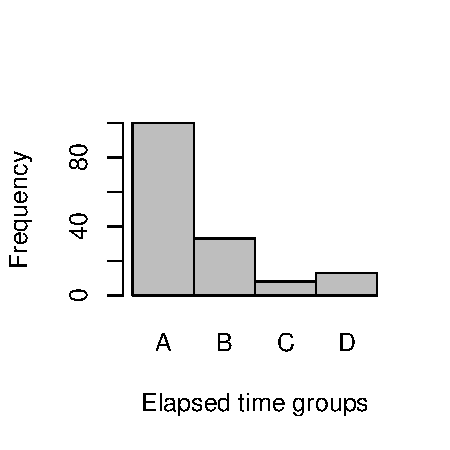
\includegraphics[width=0.5\textwidth]{plots/timecost-barplot/timecost-barplot.pdf}
        \caption{\Fix{Subjects grouped by elapsed time on test execution ($t$):
        group A ($t < 1m$), group B ($1m \leq t < 5m$), group C ($5m \leq t <
        10m$(, group D ($10m \leq t$)}}
    \end{center}
    \label{fig:timecost-barplot}
\end{figure}

